\documentclass[12pt]{article}
\usepackage[pdftex]{graphicx}
\usepackage{html}
\usepackage[fleqn]{amsmath}
\usepackage[spanish]{babel}
\usepackage{ucs}
\usepackage[utf8x]{inputenc}
\usepackage{listings}
\newcommand{\lb}{{\langle}}
\title{An elementary proof of the reconstruction conjecture}
\author{
Pepito de los Palotes
\thanks{Thanks to the editors of this wonderful journal!}
\\
}
\date{
\today
}
\begin{document}
\maketitle
\begin{abstract}
 The reconstruction conjecture states that the multiset of unlabeled
    vertex-deleted subgraphs of a graph determines the graph, provided it
    has at least 3 vertices.  A version of the problem was first stated
    by Stanislaw Ulam.  In this paper, we show that the conjecture can
    be proved by elementary methods.  It is only necessary to integrate
    the Lenkle potential of the Broglington manifold over the quantum
    supervacillatory measure in order to reduce the set of possible
    counterexamples to a small number (less than a trillion).  A simple
    computer program that implements Pipletti's classification theorem
    for torsion-free Aramaic groups with simplectic socles can then
    finish the remaining cases.  
\end{abstract}
Hola, hoy son las 2012-12-17 18:56:18 +0000 y $\sqrt{2} = 1.4142135623730951$
\begin{verbatim}
a = 4*5
b = 4*5
\end{verbatim}
\begin{equation}
\Delta =\sum_{i=1}^N w_i (x_i - \bar{x})^2.
\end{equation}
We can give an equation a label so that we can refer to it later.
\begin{equation}
\label{eq:ising}
E = -J \sum_{i=1}^N s_i s_{i+1},
\end{equation}
Equation~\eqref{eq:ising} expresses the energy of a configuration
  of spins in the Ising model.\footnote{It is necessary to typeset a
  file twice to get the counters correct.}
  
\htmladdnormallink{https://github.com/cocoa/eloquent-ruby}{https://github.com/cocoa/eloquent-ruby}
\begin{align}
a & = b \\
c &= d,
\end{align}
\begin{rawhtml}
<pre>
<span class="k">class</span> <span class="nc">Test</span><span class="p">;</span> 

  <span class="k">def</span> <span class="nf">tutu</span>
  <span class="k">end</span>
<span class="k">end</span>
</pre>

\end{rawhtml}
\begin{latexonly}
\begin{lstlisting}{language=ruby}

class Test; 

  def tutu
  end
end

\end{lstlisting}
\end{latexonly}
\begin{tabular}{|c|}
\hline

    test1\\
    test2\\
    
\hline
\end{tabular}
\section{Tipos, Clases y Módulos}


\begin{verbatim}
>> obj = [1, {:a => 2}]
=> [1, {:a=>2}]
>> obj.class                      # retorna la clase de un objeto
=> Array
>> obj.class.superclass           # retorna la superclase de un objeto
=> Object
>> obj.instance_of? Object        # determina si obj.class == Object
=> false
>> obj.instance_of? Array
=> true
>> obj.is_a? Object               # determina si obj es de una subclase de Object
=> true
>> obj.is_a? Array
=> true
>> obj.kind_of? Object            # kind_of? es un sinónimo de is_a?
=> true
>> Array === obj                  # equivalente a obj.is_a? Array
=> true
>> Object === obj
=> true
>> obj.respond_to? 'each'        # si tiene un método público o protected llamado 'each'
=> true                          # si se le pasa true como segundo argumento se comprueban
                                 # también los privados
>> Array.instance_methods(false) 
=> ["insert"
 "sort" "include?" "size" "&" "to_ary" "clear" "yaml_initialize" "shuffle"
 "replace" "pack" "zip" "flatten!" "to_s" "pop" "pretty_print_cycle" "hash"
 "cycle" "*" "indices" "nitems" "index" "collect" "+" "compact!"
 "last" "rassoc" "count" "drop" "delete" "delete_at" "combination" "collect!"
 "select" "each_index" "-" "flatten" "eql?" "fill" "length" "uniq!"
 "at" "choice" "reject!" "[]" "take" "inspect" "shift" "compact"
 "pretty_print" "[]=" "|" "find_index" "slice!" "each" "empty?" "transpose"
 "<<" "frozen?" "rindex" "map" "reverse_each" "reverse!" "to_a" "push"
 "uniq" "delete_if" "first" "product" "drop_while" "concat" "reject"
 "map!" "join" "slice" "indexes" "taguri" "<=>" "assoc" "fetch" "to_yaml"
 "==" "values_at" "permutation" "take_while" "unshift" "reverse"
 "sort!" "shuffle!"  "taguri="]
\end{verbatim}

  \subsection{Antepasados y Módulos}
  
Los siguientes métodos sirven para determinar que módulos han sido incluídos 
y cuales son los ancestros de una clase o módulo:
\begin{verbatim}
[~/chapter8ReflectionandMetaprogramming]$ cat ancestryAndModules.rb 
module A; end

module B; include A; end

class C; include B; end

if __FILE__ == $0
  puts C < B               # => true: C includes B
  puts B < A               # => true: B includes A
  puts C < A               # => true
  puts Fixnum < Integer    # => true: all fixnums are integers
  puts Integer <Comparable # => true: integers are comparable
  puts Integer < Fixnum    # => false: not all integers are fixnums
  puts (String < Numeric).inspect  # => nil: strings are not numbers
  
  puts A.ancestors.inspect         # => [A]
  puts B.ancestors.inspect         # => [B, A]
  puts C.ancestors.inspect         # => [C, B, A, Object, Kernel, BasicObject]
  puts String.ancestors.inspect    # => [String, Comparable, Object, Kernel, BasicObject]
 
  puts C.include?(B)       # => true
  puts C.include?(A)       # => true
  puts B.include?(A)       # => true
  puts A.include?(A)       # => false 
  puts A.include?(B)       # => false

  puts A.included_modules.inspect  # => []
  puts B.included_modules.inspect  # => [A]
  puts C.included_modules.inspect  # => [B, A, Kernel]
end
\end{verbatim}


\input{examples/module.tex}
\begin{figure}[htb]
\begin{center}
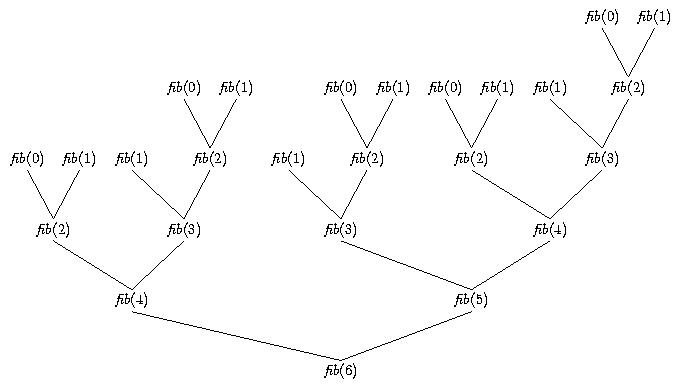
\includegraphics[scale=0.7]{examples/fibonacci.png}
\end{center}
\label{figure:fibonacci}
\caption{Arbol de llamadas para la función de Fibonacci}
\end{figure}
\end{document}
